\documentclass[12pt, oneside, a4paper]{report}

\usepackage{afterpage}   \usepackage{amsmath}     \usepackage{amssymb}
\usepackage{cancel}      \usepackage{enumitem}    \usepackage[english]{babel}
\usepackage{bold-extra}  \usepackage{booktabs}    \usepackage{caption}
\usepackage{cite}        \usepackage{fancyhdr}    \usepackage[T1]{fontenc}
\usepackage{geometry}    \usepackage{graphicx}

\usepackage[breaklinks, colorlinks=true, linkcolor=blue, linkcolor=blue,
    anchorcolor=blue, citecolor=blue, filecolor=blue, menucolor=blue,
    runcolor=blue, urlcolor=blue]{hyperref}

\usepackage{layout}      \usepackage{listings}    \usepackage{lscape}
\usepackage{makecell}    \usepackage{mathastext}  \usepackage[version=4]{mhchem}
\usepackage{multicol}    \usepackage{numprint}    \usepackage{setspace}
\usepackage{tikz}        \usepackage{times}       \usepackage{titlesec}
\usepackage{xcolor}      \usepackage{xurl}

\usetikzlibrary{calc}

% URL font
\urlstyle{same}

% \usepackage{showframe}

% Taille du tableau -0.5 cm
% \textheight = 731 pt
% \textwidth = 483 pt

\lstset{
    basicstyle=\footnotesize\ttfamily,
    emphstyle={\bfseries},
    escapeinside={(*}{*)},
    numbers=left,
    numberstyle=\scriptsize\color{black},
    tabsize=4,
    columns=fixed,
    frame=tb,
    showstringspaces=false,
    showtabs=false,
    keepspaces,
    emph={
        SI,
        SINON,
        RETOURNER,
        FIN,
        POUR,
        ALORS,
        \backslash\backslash,
        VARIABLE,
        INITIALISATION,
        TRAITEMENT,
        SORTIE
    },
    literate={à}{{\`a}}1
    {é}{{\'e}}1
    {è}{{\`e}}1
    {<-}{{$\leftarrow$}}1
}

\geometry{top = 2.5cm, bottom = 3.5cm, hmargin = 2.5cm}

\newcommand{\emptypage}{
    \newpage
    \null
    \thispagestyle{empty}
    \addtocounter{page}{-2}
    \newpage
}
\newcommand{\Chapter}[2]{
    \begin{center}
        \chapter{#1}
        {
            \Large Cours présenté par #2
            \vspace{1em}
        }
        \hrule height 2pt
    \end{center}
}
\newcommand{\fref}[1]{\hyperref[#1]{\textbf{[fig.~\ref*{#1}]}}}
\newcommand{\subfref}[2]{\hyperref[#1]{\textbf{[fig.~\ref*{#1}~: #2]}}}
\newcommand{\tref}[1]{\hyperref[#1]{\textbf{[tab.~\ref*{#1}]}}}
\newcommand{\aref}[1]{\hyperref[#1]{\textbf{[\ref*{#1}]}}}
\newcommand{\eref}[1]{\textbf{[éq.~\eqref{#1}]}}
\newcommand{\eqdes}[1]{
    \begin{footnotesize}
        \hrule height 1pt
        #1
    \end{footnotesize}
}
\newcommand{\p}[1]{$^\text{#1}$}
\newcommand{\id}[1]{$_\text{#1}$}
\newcommand{\can}[1]{$\cancel{\text{#1}}$}
\newcommand{\mathBF}[1]{\mathbf{\boldsymbol{#1}}}
\newcommand{\ms}{\\[1em]}
\newcommand{\C}{\tiny$\blacksquare$}
\newcommand{\Cite}[1]{\p{\textbf{\cite{#1}}}}

\renewcommand{\theequation}{\thechapter{}.\arabic{equation}}
\renewcommand{\headrulewidth}{0pt}
\renewcommand{\thesection}{\arabic{section}}

\newenvironment{matheq}{
    \begin{equation*}
        \begin{array}{rcl}
}{
        \end{array}
    \end{equation*}
}
\newenvironment{f}{
    \begin{figure*}
        \begin{minipage}[c][\textheight][c]{\textwidth}
}{
        \end{minipage}
    \end{center}
}
\newcounter{exempleNumber}\setcounter{exempleNumber}{1}
\newenvironment{exemple}{
    \begin{itshape}
        \vspace{.5em}\footnotesize
        \phantom{M}\hfill\textbf{EXEMPLE~\arabic{exempleNumber}}\hfill\phantom{M}
        \vspace{.5em}
        
        \hrule\vspace{3pt}
}{
        \vspace{3pt}\hrule
    \end{itshape}\stepcounter{exempleNumber}
}

\makeatletter
\renewcommand\tableofcontents{%
    \@starttoc{toc}%
}
\renewcommand\listoffigures{%
        \@starttoc{lof}%
}
\renewcommand\listoftables{%
        \@starttoc{lot}%
}
\def\tagform@#1{\maketag@@@{\bfseries(\ignorespaces#1\unskip\@@italiccorr)}}
\makeatother

\setcounter{tocdepth}{3}
\setcounter{secnumdepth}{3}

\setlength{\parindent}{0pt}
\setlength{\parskip}{0.20cm}
\setlength{\headheight}{0pt}
\setlength{\columnsep}{2cm}

\titleformat{\section}[hang]
{\bfseries}
{\thesection.}
{1ex}
{}

\titleformat{\subsection}[hang]
{\bfseries}
{\thesubsection.}
{1ex}
{}

\titleformat{\subsubsection}[hang]
{}
{\phantom{\bfseries\thesubsection\hspace{1ex}}\thesubsubsection.}
{1ex}
{}

\captionsetup[figure]{font=footnotesize, labelfont=bf, name={Fig.}, labelformat=simple}

\pagestyle{fancy}
\fancyhead[]{}
\fancyfoot[C]{--~\thepage{}~--}
\fancypagestyle{plain}{\fancyhf{}\fancyfoot[C]{--~\thepage{}~--}}

\title{Report REMC implementation}
\author{ROUAUD Lucas}
\date{\today}

\begin{document}
% \layout{}
\pagenumbering{arabic}
\begin{huge}
    \begin{flushleft}
        \bfseries Implementation of a Replica Exchange\linebreak
        Monte Carlo algorithm using Python
    
        \vspace{1ex}
        
        \hrule height 2pt
    \end{flushleft}
\end{huge}

\vspace{1ex}

\textit{\textbf{\large Document réalisé via \LaTeX{}}}

\textbf{REPORTER:} M. GELLY J.-C. and GALOCHKINA T.

\textbf{ROUAUD Lucas --- Master 2 BI}: Université Paris Cité

\vspace{2ex}

\begin{center}
    \begin{minipage}{16cm}
        \hrule height 0.5pt width 16cm
        \vspace{1ex}
        \section*{Abstract}

        \paragraph*{Background}
        THACHUK C. and \textit{al.} describe the use of a Replica Exchange Monte Carlo algorithm. It shall permit, through Dill's H/P model, the prediction of protein folding on a 2D matrix. But only for an extremely simplified case of hydrophobic amino acid or not. In this paper, we discuss how we implement this program using Python langage and why doing it in this such of manner.

        \vspace{1ex}

        \paragraph*{Results}
        When trying on small dataset, same as the one the authors used in their article, energy results are very different. This show that the effectuation of an unfavourable movement might be badly implemented, or need a huge amount of MC/REMC step.

        \vspace{1ex}

        \paragraph*{Availability and implementation}
        This paper and the corresponding algorithm with its documentation his available on an GitHub repository: \url{https://github.com/FilouPlains/PROJECT_PY_MONTE_CARLO/}

        \vspace{1ex}
        \hrule height 0.5pt width 16cm
        
        \vspace{1ex}
        
        \begin{footnotesize}
            \bfseries ABBREVIATIONS: \textit{MC~=} Monte Carlo; \textit{REMC~=} Replica Exchange Monte Carlo.
        \end{footnotesize}
    \end{minipage}
\end{center}

\vspace{2ex}

\begin{multicols}{2}
\section{Introduction}
\vspace{-1ex}

In an article, THACHUK C., SHMYGELSKA A. and HOOS H. H. talk about a REMC algorithms in a context of protein folding, following Dill's H/P model\Cite{thachukReplicaExchangeMonte2007}. Here, we implement this algorithm using Python language.

\vspace{-2ex}

\section{Materials and methods}
\vspace{-1ex}

\begin{figure*}[!b]
    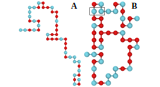
\includegraphics[width=\textwidth]{figure/conformation_example.pdf}
    
    \small
    \vspace{0.5ex}
    \hrule height 1pt

    \caption{
        \textbf{Conformation example found by MC algorithm, for a same starting sequence.} \textit{Red~=} polar residues; \textit{blue~=} hydrophobic residues; \textit{A~=} the sequence is unfold and loose energy; \textit{B~=} the sequence have one hydrophobic interaction (black square), but it appear that polar residues are "attract" inside the protein instead of outside.
        \label{f:conformation_example}}
\end{figure*}

\begin{figure*}[!b!t]
    \includegraphics[width=\textwidth]{figure/energy.pdf}
    
    \small
    \vspace{0.5ex}
    \hrule height 1pt

    \caption{
        \textbf{Graphics obtain after MC algorithm.} \textit{A~=} energy* in function of the step; \textit{B~=} bar plot of min energy obtain in function of the temperature.
        \label{f:energy}}
\end{figure*}

To implement this program, \texttt{Python 3.10.4} is used. The module \texttt{numpy 1.23} is used for vector computing and the module \texttt{tqdm 4.64.0} to show the estimate time to perform a Monte Carlo algorithm.

The probability of doing a unfavourable movement is given by:

\vspace{-2ex}

\begin{equation*}
    \left\lbrace
    \begin{array}{ll}
        1                                       & if\:\Delta{} E < 0 \\
        e^{\dfrac{-\Delta{}E}{T \times K_B}}    & else
    \end{array}
    \right.
\end{equation*}
\eqdes{with K\id{B} = Boltzmann's constant; $\Delta{}$E = energy variation between two conformation.}

While the probability of doing a replica exchange is given by:

\vspace{-2ex}

\begin{equation*}
    \left\lbrace
    \begin{array}{ll}
        1              & if\:\Delta{} \leq 0 \\
        e^{-\Delta}    & else
    \end{array}
    \right.
\end{equation*}

With Delta equal to:
\begin{equation*}
    \Delta = \left(\dfrac{1}{T_j} - \dfrac{1}{T_i}\right) \times \left(E\left(c_i\right) - E\left(c_j\right)\right)
\end{equation*}

\begin{minipage}{\columnwidth}
    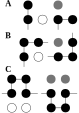
\includegraphics[width=\textwidth]{figure/move_set.pdf}
    
    \small
    \vspace{0.5ex}
    \hrule height 1pt

    \captionof{figure}{
        \textbf{All possible VSHD move set.} \textit{Black~=} Actual position; \textit{grey~=} old position; \textit{white~=} position to move next step; \textit{A~=} end move; \textit{B~=} corner move; \textit{C~=} crankshaft move.
        \label{f:move_set}}
\end{minipage}

The \fref{f:move_set} describe all implemented movement. To do so, three object where create. One that stock the coordinates, an other the amino acid and a last a sequence which enable communication those two previous one. Like that, we do not manipulate matrix which has a complexity of $O(N^2)$.

To finish, we produce a \textit{.csv} file to manipulate the data (especially energies) and optionally a \textit{.mol2} file which contains all "frame" during a movement. Like that, with a molecule visualization software like \texttt{PyMol} or \texttt{VMD}, it is possible to observe the trajectory.

\section{Results}
First, the \fref{f:conformation_example} show that conformation are sometime loose or block while doing a MC algorithm. For instance, the \subfref{f:conformation_example}{A} show that the conformation is somehow lost (like a denaturation of a protein) by a linearisation; while the \subfref{f:conformation_example}{B} show that the hydrophobic residues are going outside, which provoc a diminution of the energy. Note that those conformation are obtained at the end of a 2,000 step MC algorithm.

To continue, when we observe the \subfref{f:energy}{A} we see that the protein do not stay in local minimum, but tend to do the contrary. Also, when tacking all minimum energies values on the  \subfref{f:energy}{B}, we observe that they are not that low compare to the original article of THACHUK C. and \textit{al.}. Those observation tend to show that the algorithm search well minimum, but not efficiently and do not "stay in them".

\section{Discussion}
Firstly, the pull move was not implemented, as far as it was too complex to do so. The general method to do it to shift diagonally two residues and move their left or right followers (using recursion) until conditions are met. The first is that all amino acids have been moved until end of chain; the second is that one amino acid after movement is still at a distance of 1 of his neighbour. The thing was there's too much conditions to take in consideration, making quite hard to find a good and functional solution.

Secondly, parallelisation is never used in the algorithm. Even though the algorithm is fast, there are huge amount of time to win by doing it, especially when doing a REMC. As far as, multiple replica with differents temperature indepedent for a given number of step (until exchange if there is). For example, let's say that we have a PC with 8 cores. The program, when executing take less that 1 core. With parallelisation achieve, it's possibly a division by 8 of time's computation!

Lastly, project organisation and object communication isn't quite perfect. Not all native Python's function are well used (like magic method to work on chain list). Thus, even if, for this case, the implementation isn't that good, it's still better and faster than working with a matrix system.

\section{Conclusion}
The algorithm is indeed implement, but not perfectly at all. There's a lot of hint showing that is not good at finding global minimum and keeping the optimal conformation. You may also notice that only MC algorithm was analyze, but not the REMC. 

\section{References}
\begingroup
    \renewcommand{\chapter}[2]{}%

    % List of style here : /usr/share/texlive/texmf-dist/bibtex/bst
    \bibliographystyle{naturemag}
    \bibliography{IEEEabrv, references.bib}
\endgroup
\end{multicols}

\pagebreak
\section*{Annexes}\pagenumbering{Roman}
\addcontentsline{toc}{chapter}{Annexes}
\captionsetup[figure]{font=footnotesize, labelfont=bf, name={Annexe}, labelformat=simple}
\renewcommand\thefigure{\Roman{figure}}
\setcounter{figure}{0}

\begin{tex}
.
├── data
│
└── src
    ├── amino_acid_class
    │   ├── amino_acid.py
    │   ├── coord_manip.py
    │   └── sequence_manipulator.py
    ├── general_function
    │   ├── parsing.py
    │   └── translation.py
    ├── main.py
    ├── monte_carlo
    │   └── monte_carlo.py
    └── output
        └── output.py
\end{tex}
\end{document}
